\chapter{Discussion and Conclusion}
\label{chap:discussionConclusion}

This research has taken place against a backdrop of political and financial uncertainty for much of the UK. The two main demographics that this project engaged with---volunteer-driven heritage preservation groups, and teachers within the formal education system---have both been impacted in recent years by pressures imposed by top-down institutional policy, and funding cuts made to cope with austerity measures. In response, these groups have started to look towards more sustainable methods of utilising existing resources and novel methods of engagement. Mobile technologies clearly have a potential role in this space: their growing ubiquity in society, as well as the popularity of location-aware applications such as \textit{Pok\'emon Go}, have meant that a large number of community groups that this project engaged with were actively seeking to be represented through mobile applications. Similarly, the utilisation of mobile technologies in schools has gained popularity---both for data collection on school trips, and in the classroom for research and content creation.

This project has aimed to explore this context as a design space for mobile learning technologies which harness places---and the communities that care for them---as resources for both learning within the formal education system, and informal knowledge sharing within wider communities. Furthermore, I wanted to explore how such technologies could be used by place stakeholders to further their groups' interests and agendas, and how such mediums could be used to share their outlooks and values with new audiences. While I regard the primary contribution of this project to be the `project-based mobile learning' framework discussed in the previous chapter, another significant contribution is the set of implications for design described below: each use the above contexts and aims as a backdrop, and discuss their relation to the identified findings from the previously discussed studies. I also discuss some of the study's limitations, before concluding by responding to the research questions laid out at the project's inception.

\section{Implications for Design}

These discussions will pertain to how mobile learning technologies can be configured to support place-making, and recommendations as to how researchers and designers can better utilise the infrastructures of place as resources for civic mobile learning.

\subsection{Support Place-Making with Mobile Learning Technologies}

This project has highlighted numerous ways in which mobile learning technologies can be configured to effectively support place-making. As such, I've broken down this implication for design into six suggestions: \textit{Encourage Encounters with New Interpretations of Place}; \textit{Highlight Place Attachment \& Meaning}; \textit{Support Celebrations of Imperfection}; \textit{Promote Engagement with Communities of Practice}; \textit{Treat Mobile Learning Content as Living Media}; and \textit{Support Independent Expression \& Reflection}.

\textbf{\textit{Encourage Encounters with New Interpretations of Place:}}  Our relationships to place are molded by the experiences and familiarity we have with space. As Tuan posited: `\textit{What begins as undifferentiated space becomes place as we get to know it better and endow it with value}' \citep{Tuan1978}. Similarly, Relph argues that the process of building a relationship with space involves encountering and having experiences with it \citep{Relph1976}. Furthermore, he notes that the majority of the experiences that people had with the landscapes around them in the 1970s were mediated by machines---he noted that while it is easy to view this as a factor which acted as a barrier separating people from authentically experiencing place, technologies such as cars opened up new opportunities for people to experience spaces that had not previously been accessible to them. Today, it's evident that mobile technologies play the same role---simultaneously erecting barriers to distract people from authentic experiences in place, and opening up new opportunities to encounter places which would otherwise be too remote or abstract to be easily accessible. While we must be aware and wary of the former, the latter presents new and exciting opportunities for using technology to support place-making processes. For, unlike the automobile, digital technologies allow users to traverse more than just physical distances: they can be configured to support encountering different interpretations of place, which may not have been previously accessible (or visible) regardless of physical proximity. This project has highlighted multiple examples of how mobile learning technologies can be used to platform or celebrate others' relationships with place, such as the rangers' concerns around park funding, the heritage forum's valuing of preservation and restoration of often inconspicuous locations, and the memorandum of the local impact of prior events, such as the miners' strikes or World Wars. While such place-making interactions can be supported by non-mobile technologies (for example, the use of Google Earth VR by Jeff Gerstmann discussed in Section \ref{sec:TechMediator}), the use of mobile learning technologies can also support the ability for remote place `visitors' to respond to activities through the use of their own space/place context. For example, in Chapter \ref{chap:student-created} a student suggested creating and exchanging OurPlace Activities with other schools---using the app to compare and contrast their lived experiences with other people's, via a place they are remotely encountering. 

\textbf{\textit{Highlight Place Attachment \& Meaning:}}  As Tuan argues, people who inhabit the same physical space may, due to differing past experiences, associate the space with different meanings and values \citep{Tuan1978}. Giving stakeholders opportunities to share these experiences with others can make their understanding of a space as a place less abstract, and help them understand what makes that place special. I argue that the studies presented in this dissertation have demonstrated that mobile learning technologies such as OurPlace can be used as platforms to offer these opportunities. These studies showed how the creation of mobile learning activities can give opportunities for highlighting and sharing \textit{place attachment} and \textit{place meaning} \citep{Kudryavtsev2012}. Place attachment---the degree to how much someone values or identifies with a place, due to it fulfilling their needs or defining them as an individual---was demonstrated through the use of the app by park volunteers in Chapter \ref{chap:Community} to highlight their group's efforts and attempt to recruit new members. Meanwhile, place meaning---the meanings that individuals ascribe to settings that they are familiar with, reflecting their environment, social interactions, culture, politics, economics and history---was seen through the use of the app to discuss notable figures in local history in Chapter \ref{chap:Teachers}, and by the Showchildren in Chapter \ref{chap:student-created} to introduce their ways of life. This is not unique to OurPlace: another example is Balestrini's CrowdMemo project, during which a mobile technology acted as a platform for community storytelling \citep{Balestrini2014}. As with Crivellaro's walking trail \citep{Crivellaro2016}, the mobile nature of OurPlace also supports genuine engagement with the environment, with many of the app's Task Types encouraging learners to pause and reflect in-situ. I argue that the deliberate exposition of these factors through technology introduces opportunities for learners to interpret others' place-based experiences: informing their own place-making process with the values of other stakeholders.

\textbf{\textit{Support Celebrations of Imperfection:}} Using mobile technologies to highlight place attachment and meaning could be particularly useful when used in places which are `under appreciated'. For example, during the ParkLearn workshop covered in Chapter \ref{chap:Community}, volunteers referred to the value they held in the imperfections (such as generations old graffiti) of the places they cared for. In some cases, making these safe or suitable for physical public access could sanitise them, eradicating what made the places special to the stakeholders in the first place. In these instances, learning technologies offer a potential solution: allowing people to remotely experience place they cannot physically access, supporting the building of vicarious insideness and support for preservation. More subversively, the grassroots nature of OurPlace's Activity creation process could also allow unofficial support for people entering these areas unsanctioned (something which the participants reported happened anyway). The ability to remotely open up these places without the need to sanitise their value could help counter Relph's concerns regarding `placelessness': `\textit{the casual eradication of distinctive places and the making of standardised landscapes that results from an insensitivity to the significance of place}' \citep{Relph1976}. This project's findings support those of Crivellaro \citep{Crivellaro2016}, suggesting that while content created top-down by institutions and local government would often be incentivised to present a sanitised interpretation of place, granting stakeholders direct control of the content creation process may result in a more authentic, `warts and all' representation based on lived human experience.

\textbf{\textit{Promote Engagement with Communities of Practice:}} A key advantage of mobile learning technologies is that they allow for users to engage in authentic learning contexts---in both the humanist geographer sense that they can provide `genuine experiences' through unmediated access to place's social qualities and constructs \citep{Relph1976}, and also in the learning sciences sense, where Situated Learning Theory posits that learning frequently occurs through legitimate peripheral participation in communities of practice \citep{lave1991situated}. Through supporting communities of practice in creating and sharing learning resources, mobile learning technologies make it easier for newcomers to engage in peripheral participation with those communities. Emphasising this link between the learning resources and the individuals and communities which create them further encourages the place-making process: learners are exposed to others' place attachment and place meaning, while also forging their own experiences in place via the technology medium. This exposure to communities of practice may not be immediately obvious to the learner---for example, the rangers and volunteers in Chapter \ref{chap:DesignSpace} aimed to nurture an appreciation of their place within the schoolchildren, rather than recruit them as volunteers. Sometimes this may be more explicit, as in the case of the `Talking Statue' project, where the OurPlace Activity included Information Tasks which described the volunteer group's work and how the user could get involved. However, even this was obscured behind the Activity's primary goal of delivering historical information about the park's heritage.

\textbf{\textit{Treat Mobile Learning Content as Living Media:}} The combination of mobile hardware, wireless networking and easily configurable software enables these communities of practice to design and create novel interactions for use by others within an authentic learning environment. In this regard, OurPlace Activities could be classed within the scope of `cross-media interaction', as posited by Giaccardi et al \citep{Giaccardi2008}. They argue that the use of multiple forms of media and technology can create new forms of socio-technical infrastructure, allowing place-making through new cultural experiences and the exploration of people's relationship with place. Giaccardi et al. also argue the importance of making heritage a `living practice' through repeated interactions over time, where people are given `\textit{active and supportive roles, [engaging] them in connecting to each others’ experiences, considering each other’s interpretations, and building insights that may lead to new meanings and relationships.}' The use of OurPlace within schools shows how this might be put into practice, with the local heritage around each school acting as each class's focus for both research and creativity. The nature of digital content and school cohort systems also encourages this to be an ongoing, living practice: where each class experiences and builds upon the previous class's local heritage research. 

\textbf{\textit{Support Independent Expression \& Reflection:}} As McCarthy and Wright argue, mobile phones and tablets are intrinsically personal devices which are particularly well suited to allowing for private encounters in public space and `\textit{blurring the traditional boundaries between public and private, intimate and extraneous}' \citep{McCarthy2005}. They argue that technologies which engage people on a personal level can help them feel `in place'. This focus on the individual experience of using technology can allow for explorations of private interpretations of place within public space. For example, RIOT!1831 allowed participants to privately experience an interactive play whilst in an authentic, yet public, space \citep{Blythe2006}. Similarly, Google Earth allows for the exploration of personal experiences in a virtual, dream-like representation of real public spaces, with some of the more abstract elements being up to interpretation \citep{Gerstmann2016}. Some of the usage of OurPlace mirrored these aspects of private experiences in and building of place: for example, one of the heritage workshop participants considered using OurPlace to subvert the usual bureaucratic system in place for choosing commemorative plaques, instead creating their own personal set of digital plaques independently. Other instances could be seen in schools' use of Activities, where students would retreat away from the main group to be able to record their thoughts and reflections without being interrupted or overheard. This focus on the individual is an important part of OurPlace---while many of the engagements involved participants creating Activities as a group, the application maintains the ability for individuals to use the technology as a platform for self expression within place, be that through creating their own Activities or responding to others'. Relph argues that by focusing on wider representation rather than recognising and representing individual viewpoints, we run the risk of highlighting an inauthentic identity which no longer represents anyone \citep{Relph1976}. However, Relph also warns that place can be misrepresented, either by those who are invested in its success or blind to its flaws---creating a more palatable, `disneyfied' ideal. Studies such as those held by Crivellaro et al. might suggest that this is best combated by opening up the ability for all individual stakeholders to create and share materials regarding their lived experiences \citep{Crivellaro2016}. However, this does not account for the fact that stakeholders cannot share what they do not know, and so may inadvertently create materials which do not give a complete representation of place. For example, Teacher 5's class created Activities relating to slavery abolitionists who had had a presence in the area---it is generally accepted that the North-East of England was a mainstay in the country for the abolitionist movement. However, the children were not aware that there had also been major businesses in the area that profited from the slave trade, including refineries of slave produced goods such as sugar and even ironworks which supplied slave restraints and plantation tools \citep{LitPhil2007}. While much of the point of OurPlace is to allow for individuals to share personal interpretations of place (by definition subjective, and not impartial), these created Activities could be argued to give an incomplete (and rather charitable) representation of the place's heritage with regards to its relationship with slavery. I argue that this highlights a need for designs that promote thorough research amongst content creators, and critical reflection on the part of consumers of these generated materials.

This project has highlighted that place-based mobile learning technologies can be useful tools for supporting place-making processes. While many digital technologies can open up new opportunities for encountering place, mobile technologies are unique in that they offer the ability to also do this in authentic physical \textit{and} social contexts, which has been argued to strengthen the learning and place-making experience. I argue that this project has demonstrated that technologies such as OurPlace can take this a step further: by supporting all users as creators of place-based mobile learning materials, OurPlace can also be used to highlight the place attachment and place meaning held by stakeholders, both as individuals and in communities of practice. These materials can act as new layers of socio-technical infrastructures which grant visitors new opportunities for encountering place through novel interactions on a personal level. In this project, these technologies have been shown to have the potential to highlight place elements whose place stakeholders feel are underappreciated, to subvert the limitations of top-down institutions, and to allow for the sharing of lived experiences within place. However, representing place through mobile learning technologies can present the same potential pitfalls as other mediums, particularly when it comes to authentic and complete representation. To combat these issues, I would recommend future work in this space investigate how technology designs can promote critical reflection and assessment in the creation and consumption processes of mobile learning technologies.

\subsection{Meaningfully Engage with Authentic Learning Contexts}

In order to support authentic learning experiences, the intricacies and individual elements of each context must be taken into account. During his discussions of the issue of `placelessness', Relph argues that the elements which make places distinct must be recognised and valued \citep{Relph1976}. He asserts that if we are overly concerned with designing efficient solutions which are interchangeable between different contexts, they cannot fully take advantage of the value of place. If these indistinct systems treat place as an anonymous, interchangeable factor, they can only offer `inauthentic' experiences of place and risk normalising such experiences within society. It's possible to view OurPlace through this lens: the application acts as a generalisable tool, which can be applied in almost any context. It's also possible to make OurPlace Activities which do not relate specifically to any particular context: like other examples such as Khan Academy or Wikipedia, Frohberg would label these as `context independent' learning experiences within the Task Model for Mobile Learning \citep{Frohberg2009, Taylor2006}. 

\begin{figure}
\centering
  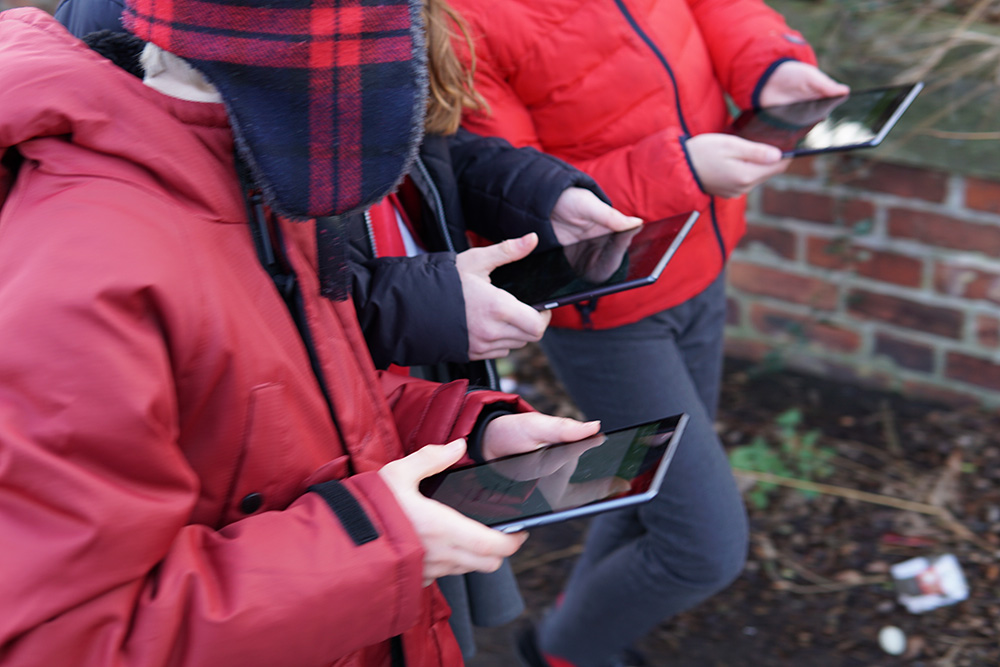
\includegraphics[width=0.85\columnwidth]{images/chapter09/senseExplorers.jpg}
  \caption[Students use OurPlace to record environmental readings from their high street]{Students use OurPlace to record environmental readings from their high street during the Sense Explorers project.}~\label{fig:senseExplorersHighSt}
\end{figure}

However, I argue that it is not just the generic OurPlace toolkit itself which provides the learning experience: it is the Activities which are created using these tools, and these can offer a wide variety of relationships between the Activity creator, the learner and the technology medium. For this reason, created Activites should be assessed by their own merits, separate from the application itself. For example, the easiest of Frohberg's other context types to implement through OurPlace is to have the learning activity have a \textit{physical} contextual relationship with the learner: the Activity takes place in a space relevant to the learning topic, meaning it is authentically situated in physical space. Rather than simply have the learner passively absorb material, OurPlace also supports a degree of learner interactivity within this authentic space---Task Types such as \textit{Location Hunt} react to the learner's physical location as an input method, whilst \textit{Map Marking} Tasks can give the learner a degree of agency in that they themselves choose the locations of interest. An example of an Activity which is based in a physically authentic context would be the park volunteers' `talking statue', which lectured the learner about the history of the learner's location, before guiding them around the park with \textit{Location Hunt} Tasks. These Activities can also be configured to support a `reconsideration' of places with which the learner already has a relationship: for example, the \textit{Sense Explorers} OurPlace Activity asked students to reflect on the environmental factors of the areas surrounding their school (Figure \ref{fig:senseExplorersHighSt}). Doing this in familiar places contextualised the environmental issues the students encountered, removing a degree of abstraction and supporting a re-examination of place with new context.

Furthermore, OurPlace Activities can also take place in what Frohberg labels as an authentic `social learning context': where learning occurs not just in authentic space, but authentic place---through the sharing of relationships with other community members and even entering communities of practice \citep{lave1991situated}. This social learning context is often much more personal, with content being driven by the values of the context's stakeholders. Examples of this within the OurPlace studies include its use within the \textit{Tyne Fresh} project and its use during the Travelling Showmen school trip. In both of these, the OurPlace Activity was used as a way to structure the school students' engagements with local stakeholders: promoting in-situ reflection not only in authentic space, but also through social engagements with local stakeholders---each of whom had values, knowledge or heritage to share. As such, I believe that OurPlace can be used as an effective tool for learning in multiple (independent, formalised, physical, social) learning contexts, and as shown in Chapter \ref{chap:Teachers}, seamlessly transition across these contexts when needed.

However, this obviously hinges entirely on the content created for the application---as suggested in Chapter \ref{chap:DesignSpace} and evidenced in Chapter \ref{chap:student-created}, without a strong contextual focus the technology itself can inadvertently become the learning objective, detracting from the learner's experience in place. As the technology itself doesn't have a meaningful relationship with the infrastructures of place, it can't supply the knowledge, values or social tensions needed for insightful learning experiences in space and place. This was somewhat alluded to during the heritage workshop in Chapter \ref{chap:Community}, where one of the participants was disappointed that the Activities took the structure of a traditional school worksheet---a teaching method disliked by both Teacher 5 and Blumenfeld due to its detachment from real-world, authentic learning contexts \citep{Blumenfeld1991}. Without Activity creators contributing their knowledge or beliefs, OurPlace can only offer these shallow learning experiences. Because of this, I frequently struggled to create Activities which demonstrated the OurPlace app's capabilities in a meaningful way: I lacked the necessary passion, knowledge and stakeholder insights about the place at hand to create worthwhile Activities about them myself.

For these reasons, the creation of insightful content about the place in question is doubly important. Through the `Community Historians' project, Fox and Le Dantec demonstrated the importance of involving and emphasising the agency and perspective of community members from the project's outset, as they were the ones best positioned to inform the final design \citep{Fox2014}. With this in mind, they re-framed the community members, demonstrating their importance and agency within the research by referring to them as `community historians' rather than `participants'. The same can be said of utilising the knowledge, passions and agendas of local stakeholders for creating OurPlace Activities. However, the community historians were still collaborators who had been approached by the research team, rather than start a movement of their own inclination. The goal of OurPlace was to take this a step further, and provide a DIY solution to support stakeholders in creating place-based mobile learning activities as they saw fit, without the need for institutional support (including the research team).

By this metric, the success of some of the created Activities is debatable---very few groups created full Activities without any intervention on our part beyond sharing the app's existence (the lighthouse discussed in section \ref{app:lighthouse} being the main example), with a number of other groups seemingly stopping after creating Activities to test how the system worked. In order to promote meaningful engagement in authentic learning contexts, I recommend that designs for place-based, mobile learning technologies utilise the unique qualities of the spaces and places in which they operate. While engaging with the infrastructures and physical elements of space may be relatively simple, this project has shown that utilising place as a resource has been shown to be much more difficult. Doing so requires significant input from local stakeholders in order to take advantage of their knowledge and passions: creating content without them risks inauthentic representations of place, fewer opportunities for learners to engage with new communities of practice, or even a learning experience which concentrates more on the medium than the learning objective. 

\subsection{Provide Value to Stakeholders}

Getting this input from local stakeholders is not a given---while simple OurPlace Activities can be made in mere minutes, the best ones are those which have been well thought out, thoroughly researched and even tested and iterated upon. As such, the production of these learning materials can require stakeholders to volunteer a significant amount of time, energy, and---if they are not particularly comfortable with digital technology---step outside of their comfort zone. For these reasons, it's become clear over the course of this project that this can not be a one-way contribution of resources: if they are to invest this effort, the stakeholders need to get something back out of their engagements with the technology.

The most obvious (and likely most commonly effective) of incentives is that of resources: OurPlace was seen as an appealing and viable option for many of the participants we engaged with, with it being free to use being a major contributing factor. As participants noted in the Heritage Forum workshop (Chapter \ref{chap:Community}), commissioning custom mobile applications can get extremely expensive. This is compounded by the fact that not only were the groups we engaged with frequently underfunded or entirely volunteer-driven, but simply having a mobile application doesn't mean that people will engage with it---at least, enough to justify the financial investment. As a result, OurPlace was seen as a low-risk option. While financial incentives are an obvious observation, it seemed to nevertheless be an influential factor.

One of the themes identified during this project was that granting both learners and stakeholders greater degrees of control over the content they produce can lead to a sense of ownership over it. This in turn seemed to galvanise the creators into sharing their content with others---for example, the `talking statue' park volunteers immediately shared their Activity through as many channels as they could (including the local newspaper), and nearly all of the school groups had children showing their creations to both their peers and teachers alike. As with our engagements with community groups during the OurPlace project, Balestrini et al. note that their participants' high levels of engagement with CrowdMemo was likely largely due to the community's significant and pro-active involvement with the conception and running of engagements \citep{Balestrini2014}. This mirrors the use of OurPlace by many of the stakeholder groups, who often initiated any use of the app and had creative control over the Activities they produced. However, Balestrini et al. also note that a sense of ownership is not always enough to sustain engagement with a project over time, and argue that a sustained engagement with the participants was achieved by providing value to all of the involved stakeholders---with this value being provided in ways varying from simply respecting and valuing the participants' lived experiences, to providing opportunities for them to learn new skills. While not strictly a part of the technology, I believe that extensively working with and within groups such as the Heritage Forum supported this process for OurPlace: it allowed the research team to identify ways in which we could provide value to the collaborators in return for their own contributions. The benefits of this kind of collaboration are also highlighted by Fox and Le Dantec, who found that configuring their research approach to be clearly and immediately advantageous to the community members greatly increased engagement \citep{Fox2014}. The extent of this collaboration was demonstrated by the re-framing of participants to `Community Historians', avoiding language which implied an unequal power dynamic between the community and the research team.

Another key consideration is if the technology is able to empower the stakeholders through the promotion of individual/group agency. I believe that this is another area where it is an advantage that OurPlace's Activity creation process is ran independently of any institutions or researchers: by this being a self-directed process, stakeholders are able to act as free agents, configuring their created Activities towards meeting their own requirements and supporting their own agendas. Previous HCI works have examined how other types of creative technologies which support `Do It Yourself' approaches can promote individuals' agency \citep{Chatting2017, Meissner2017}. In their review of literature noting indicators of individual agency and empowerment, Ibrahim and Alkire describe agency as `\textit{a kind of process freedom}', noting that other authors describe agency as being `\textit{the ability of an individual to set [their] own goals and act upon them}', and that agency can support the acquisition of `power resources': the assets which can be accumulated, invested and exchanged for `power' \citep{Ibrahim2007}. Rowlands defines power as being in four categories: power \textit{over} other objects or people, describing the ability to manipulate or resist manipulation; power \textit{to} do new things with new possibilities; power \textit{with} a group acting with a common interest; and power \textit{from within}, a measure of respect, growth and acceptance for oneself and others \citep{Rowlands1997}. 

I argue that parallels can be drawn between these factors and the use of OurPlace within several of this project's studies. For example, the park volunteers were able to fulfil their goal of creating a `talking statue' (as described in Chapter \ref{chap:Community}), (mostly) independent of the usual top-down institutional restrictions which would have affected their creative control and output. In this instance, I argue that Activity authorship acted as a power resource for the volunteers: it allowed them (power \textit{with}) to create their own content as they saw fit (power \textit{to}) and release it in their own timeframe, with a minimal need for top-down assistance from the local council (power \textit{over}). The platform being open source (and therefore available for stakeholders with the knowledge and inclination to reconfigure to suit their own needs) also gave one heritage workshop attendee an opportunity to modify the application, allowing the reconfiguration of the software into a more suitable power resource. Arguably, instances such as the art trail volunteer gaining enough confidence to procure and learn how to use their first smart device are also examples of power \textit{from within}. In this regard, I believe that mobile learning technologies are able to empower users through content ownership, giving them a meaningful benefit to contributing time and energy towards content creation. In OurPlace, this was achieved by granting more creative control to users and elevating them from consumers to producers of educational content.

\section{Responding to the Research Question and Objectives}
\label{sec:RespondingtoQuestions}

At the outset of this document, I presented this research question as the main instigator for the research project:

\begin{displayquote}
\textbf{How can mobile learning technologies better surface and utilise the civic value of places and empower the communities which give them meaning?}
\end{displayquote}

This question was then extrapolated into three more manageable research objectives, each with a more focused scope. I will now respond to each of these in turn, given the findings of this research project.

\begin{displayquote}
\textbf{Investigate how existing place and community infrastructures can be better utilised as resources for mobile learning.}
\end{displayquote}

Through this project, I found that it was possible for mobile technologies to assist teachers in making use of existing infrastructure as learning resources. Furthermore, rather than just simply engaging with the surrounding \textit{physical} resources, technologies such as OurPlace can be configured to support engagements with other, less tangible and immediately obvious qualities of place---the social elements such as heritage, politics and other relationships with local communities which turn spaces into places. 

As suggested by previous research, this is best done through hosting learning activities within authentic physical and social learning contexts. While many mobile learning technologies successfully engage with physical contexts (i.e. the learning takes place in a space relevant to the learning topic---the learning is physically authentically situated), relatively few take full advantage of place as a learning resource by also engaging with its social context, in which learning occurs through forming relationships with others in place (e.g. engaging with communities of practice). 

In this project, this was attempted in two ways: having the place stakeholders share their knowledge and outlooks through the creation of educational materials for others to experience and respond to; and, secondly, having the mobile learning component exist as a part of a larger learning project, giving students the time to research a place before using the technology within the authentic learning environment. This necessitated the inclusion of a seamless mobile learning technology, which would allow the learning experience to follow the learner across multiple contexts (e.g. classroom activities, then field trip, then follow-up classroom activities). 

However, in many contexts this is easier said than done. For example, while many of the primary schools we engaged with were able to dedicate the time conducive to these more holistic styles of learning, the secondary schools were much more time limited, due to obligations to prepare students for quantitative assessments. For this reason, a framework to guide the use of mobile learning technologies within place-focused, project-based learning activities was developed---one which could be reconfigured in order to adapt to the contextual challenges of a given learning environment. While such adaptations will frequently result in compromises to the final learning experience, structuring such projects through the use of such a framework allows for outcomes to be more predictable and manageable. 

\begin{displayquote}
\textbf{Explore how mobile learning technologies can be designed to promote civic learning.}
\end{displayquote}

For the purposes of this research project, civic learning has been defined as being that which supplies the learner with the knowledge, skills and values they need to be citizens who actively participate in their local communities and take responsibility for understanding and improving them. This project has highlighted a number of ways in which civic learning can be promoted, with nearly all of them being related to supporting place-making: the process of forming relationships with space through having personal experiences with it, ergo forming place. Through developing a relationship with place, learners might be able to gain an appreciation of its value, potentially (as hoped by some of our volunteer groups) leading to a degree of stewardship.

We found multiple ways in which mobile learning technologies can be configured to promote place-making. One of the most important was to give learners a a greater degree of control over their learning activities. Not only did we find that students were more engaged with learning activities which involved greater degrees of creativity and decision making, but this greater degree of control also supports learners in gaining their own personal experiences with place---allowing them to form their own unique interpretations and relationships. Furthermore, besides the obvious advantages of supporting learning being authentically situated in the relevant place, mobile technologies can also support in-situ reflection on top of simple data collection and absorption of knowledge. By supporting reflection in-place rather than it happening upon return to the classroom, the technology can be used to maximise the amount of the learning process that takes place within the authentic environment.

OurPlace also supported place-making by making it easier for learners to encounter other stakeholders' interpretations of place. Gaining additional perspectives on a place and awareness how different stakeholders' relationships with it differ could help learners gain a deeper understanding of a place's value. Furthermore, this functionality makes it possible for learners to be introduced to stakeholder communities of practice, offering further vectors for additional understanding and opportunities for active participation.

\begin{displayquote}
\textbf{Explore how mobile learning technologies can be designed for the empowerment of place stakeholders.}
\end{displayquote}

I argue that a key way in which mobile learning technologies can empower local stakeholders is by acting as tools which stakeholders can use as a means to fulfil their own personal, place-based agendas. However, doing this effectively requires designers to both identify these agendas, and produce designs which will work effectively within a stakeholder's given context. As seen in existing research \citep{Fox2014, Crivellaro2016}, spending time to work closely alongside place stakeholders can assist the research team in identifying their needs and agendas. In this project, having an active and co-productive relationship with stakeholder groups greatly assisted in the design process, as I was able to gain a greater understanding about the group's motivations, strengths and weaknesses, resulting in the development of a more suitable technology design. 

For OurPlace, this meant designing a technology which emphasised stakeholder agency. During these studies, stakeholders were able to create their own bespoke, interactive mobile learning activities, independent from the top-down institutions (such as local government) upon which they are normally reliant. In this regard, OurPlace was able to empower these stakeholders in sharing their knowledge and agendas by giving them a means of production within their own control, without the need for technical knowledge or significant funding. I argue that for these volunteer stakeholders, the ability to create their own mobile learning activities acted as a power resource: it allowed them to create their own content as they saw fit and release it in their own time-frame, with a minimal need for top-down assistance from the local council. This can also be seen in other Digital Civics-related projects, such as PosterVote \citep{Vlachokyriakos2014} and AppMovement \citep{Garbett2016}. In line with these examples and the findings of this project, I would recommend that designers looking to empower place stakeholders through mobile technologies explore how such technologies could support stakeholders in attaining greater degrees of agency in fulfilling their own needs and agendas.

\section{Project Limitations and Future Work}

While this project involved engaging with dozens of stakeholder groups and hundreds of school children, the work still faced a number of limitations which could be explored in future work. This section will address the project's most major limiting factors.

\subsection*{Measuring Learning and Curriculum Integration}
One of the choices made from the project's inception was that we would not take measurements of learning outcomes. While this might seem strange (OurPlace is, after all, a tool for creating and consuming learning resources), the subject of assessing students' learning is large enough that it would have taken up a significant portion of this document and research time. As this is such a huge topic, a significant body of work already exists investigating the quantitative and qualitative benefits of outdoor learning, technology-enhanced learning and project-based learning pedagogies. Rather than measure knowledge before and after the use of the platform and include control groups, I decided to trust the teachers' judgements in how each engagement went---how the students performed, how well they engaged with the learning activities and how well the application integrated into the teaching environment. This seemed like the optimal choice, as the teachers had an extensive understanding of the students' past performances, as well as a thorough understanding and experience with teaching and assessing for various pedagogies. In this regard I positioned myself as a layperson, supporting the teachers in using the OurPlace platform in ways they saw fit, and enquiring about their opinions during and after each study.

As denoted by the project's design goals, rather than directly influence learning outcomes by itself, I designed OurPlace to support a variety of types of engagement and learning (i.e. authentic, situated, seamless, project-based) that have been previously shown to increase the probabilities of learning happening \citep{Frohberg2009, Sharples2013, Blumenfeld1991}. As such, OurPlace's evaluation was based on demonstrating that these types of engagements happened, rather than measuring students' academic achievement. As such, by promoting these engagements, I argue that OurPlace increased the probability of meaningful learning occurring. Such an approach has been taken by previous researchers (e.g. \cite{kharrufa2010thesis}) who have focused on less easily quantifiable---but still recognised and valued---skills such as critical thinking, meta-cognition and reflective thinking. Similarly, this project was largely focused on growing an awareness of the value of place, and the communities, heritage and environment that form together to make it. This placed a significant focus on holistic approaches to learning, which tend to run counter to quantitative measurements and formal examinations due to their focus on emotional development, social skills and critical thinking, rather than simple fact-based and rote learning. Measuring the outcomes of such learning processes tends to be less concrete, and so this was approached through observation and conversation, rather than formal examination.

That said, not every school can follow this type of learning approach---either due to teaching preferences or institutional pressures. For example, School 3 was particularly focused on `teaching to the test'---secondary schools are particularly pressured to perform well during exams, leading to a very narrow curriculum focus. This leaves little room for holistic teaching approaches, as methods which don't require learners to remember facts related to examination criteria are often perceived as being `risky'. We struggled to get many other secondary schools to take part in the project for this reason, and those which did, such as School 2, were only for very short periods of time. This severely limits the amount of meaningful engagement that the students can have with either the technology, subject matter, or both---the lack of time resources available to the teacher would require significant compromises in PBML-like activities (see Figure \ref{fig:PBMLradar} for an illustration of compromises). For example, the \textit{Journey Through Tyne} project provided excellent opportunities for students to gain a holistic understanding of the subject matter, but the lack of classroom preparation time meant that the integration of technology was extremely shallow.

There exists an opportunity for future work to further explore how project-based mobile learning can be more deeply integrated into existing curricula, supporting elements such as formal assessments for schools which require them. I believe it's only by trying to accommodate for these requirements that we can gain meaningful insights into how PBML can fit into the practices of wider school systems. 

\subsection*{Varying Learning and Stakeholder Domains}

While this project engaged with a large number of schools and community stakeholders, these studies largely concentrated of the learning domain of local history and heritage. I believe that place and project-based mobile learning has the potential to be used in a wide variety of learning domains, with place and community infrastructure used as rich learning resources. Examples of these other domains could include: music, where schools were able to utilise local expertise to enrich their music lessons as seen in Remix Portal \citep{Dodds2017}; politics, with students investing the impact of policy upon their area by collecting various stakeholder views, \`a la Community Conversational \citep{Johnson2017}; and the sciences, exploring topics such as the impact of climate change and pollution upon the community's health in a manner similar to Sense Explorers (discussed in Chapter \ref{chap:Teachers}). There are clearly a wide number of potential application areas for PBML still to be explored.

However, while the PBML framework is tool agnostic and should be largely suitable for these different knowledge domains, it is unlikely that the same technologies that worked well the context of local heritage would perform as well when applied to others. For example, in its current form, OurPlace would likely not be an effective tool for learning music production beyond its capacity for data collection in the Research stage. If new mobile technologies need to be developed for use within these contexts, it is likely that the researchers would benefit from a process similar to what was undertaken with this project---meeting, spending time with and forming relationships with multiple relevant stakeholders (e.g. teachers, local musicians) to gain a better understanding of their needs. This process needs to be particularly thorough if it is to account for stakeholders' variations in perceptions of place---as Tuan argues, because a person’s place attachment is formed based upon individual experience, peoples' perceptions of place may not align with each other, running the risk of inappropriate design decisions if not handled with care \citep{Tuan1978}.

\subsection*{Avoiding Inadvertently Supporting Austerity Measures} 
\label{sec:InadvertentlySupportingAusterity}

As discussed, this project took place as a part of the Digital Civics agenda, set against a backdrop of economic austerity enforced by Conservative politics. I maintain that the goal of Digital Civics is to strengthen relationships between citizens and local service providers, by empowering citizens to have more involvement and agency within their government’s processes. However, this doesn't mean that technologies designed and created for this purpose can't be misappropriated and used to justify austerity measures, through cost reduction and automation. Unfortunately, the possibility for OurPlace to be misused was highlighted in the `Places in Transition' study, where the participant institutions saw value in the app as it was more economically viable than human tour guides. I don't believe that there were other instances during these studies where the app could be argued to have been used as a tool to support `down-sizing' (in fact, OurPlace technically created a job with the Community Railway Partnership), but it was concerning none-the-less. I would like to see future Digital Civics projects to critically explore how (or if) these new processes and technologies can be designed to mitigate hardships inflicted by austerity measures in a way which can't also be used to legitimise them.

\subsection*{Interventionism and Replicability}

As Dourish notes, the role of the researcher within long-term engagements with stakeholders (e.g. through ethnography) necessitates more than logging data: there is a degree of individual interpretation on top of simple observation \citep{Dourish2006}. As a result, he argues that the findings of ethnographic studies often implicitly reflect the researcher.  Likewise, design-based research requires a degree of interventionism on the part of the researcher, in order to follow a pro-active research agenda. It is highly unlikely that the events reported in this study would have happened without my numerous interventions---examples include how I supported the existence of many of the deployments through supplying classes with Android tablets; how I assisted park volunteers with creating their Talking Statue in the ParkLearn app; how I introduced the PBML framework to the teachers and ran numerous sessions; and how Open Lab supported the Travelling Showmen study by paying for transportation from School 5 to the fair. These interventions took place in naturalistic research contexts and were largely successful, but they did not naturally occur. This is an important distinction, impacting some contexts more than others: it's unlikely that the tiny School 4 could have afforded to buy a dozen Android tablets, for example.

Furthermore, the context-focused nature of design-based research means that many of the conditions and findings in this study would be hard for other researchers to accurately replicate. It is highly unlikely, for example, that a peer would be able to find teachers and schools existing in the same socio-economic, professional and political context, along with classes who shared the same attitudes to learning as those found in this project. As such, many of the specific findings are not particularly generalisable, and nor should they be: they are wrapped up in individuals' interpretations and relationships with the places and communities around them. Removing this context from the findings would simultaneously remove much of their intrinsic value. Instead (as discussed in Section \ref{sec:ResearchApproach}), this thesis has attempted to present, develop and test theory, supporting its use in other works through rich accounting of the interventions and engaged contexts to support transparency and an understanding of \textit{why} results occurred---not just \textit{what} occurred. I hope that this has been successful.

\section{Conclusion}

The primary goal of this research was to explore if and how mobile learning technologies could be used to surface the value bestowed upon local places by the communities which give them meaning: both for the purpose of education, and for the empowerment of those communities through the platforming of their values and agendas. Through holding a number of longitudinal and short-term case studies with teachers, students and community stakeholders, this project identified and explored the design space for mobile learning technologies which harness local, place-based resources (both social and physical) to support educational activities and the sharing of local knowledge and values. 

Having identified the design space for the use of public places as infrastructure for civic mobile learning, I designed and developed `OurPlace' to aid in its exploration. OurPlace is a seamless mobile learning application which supports the grassroots creation, sharing and completion of interactive, place-based mobile learning content. Through a design-based research approach, OurPlace was deployed and evaluated in authentic usage contexts, including a wide variety of schools and a number of local volunteer-based heritage groups. Varying between one-off studies and collaborative relationships which ran over multiple years, these engagements informed the evolution of OurPlace from a prototype application to a platform which has been adopted by external stakeholders.

These engagements highlighted that mobile technologies could not only be used to make use of physical local spaces as learning resources, but that the socioeconomic infrastructures of \textit{place} could also be utilised to offer learners rich insights into what gives those spaces meaning to local communities. This project found that mobile learning technologies could support learners in building relationships with place, by giving local stakeholders opportunities to share their knowledge and values and supporting learners in exploring these interpretations and concepts within authentic learning environments. I also argue that mobile learning technologies such as OurPlace can empower local stakeholders by acting as tools through which they can fulfil their own personal, place-based agendas---without needing top-down support from larger institutions, which may have their own conflicting interests.

To further explore how these findings could effectively be put into practice within formal education contexts, I introduced a framework for `Project Based Mobile Learning': a framework for a series of educational activities which engage with local place, and result in the production of student-created mobile learning content. This framework was developed over the course of a number of school engagements through a design-based research approach, and required adaptation to each school's unique contextual restraints. I demonstrated how through this framework, OurPlace and other mobile learning technologies could be used to support place-based learning through project-based pedagogies within formal education contexts, but also that any adjustments made to the framework to accommodate for contextual requirements will result in trade-offs which may impact its effectiveness in predictable ways.

These explorations have also raised new avenues for investigation in future research. In order for a wider variety of schools to benefit from these findings, further work needs to explore how project-based mobile learning can be more deeply integrated into existing curricula, supporting required elements such as formal assessments. Furthermore, in order to combat the spread of incorrect (or incomplete) information, I would recommend future work in this space investigate how technology designs can promote critical reflection and assessment in the creation and consumption of mobile learning content. Finally, I would like to see future projects critically explore how technologies such as OurPlace, which are designed to mitigate hardships inflicted by austerity measures, can be misused in ways which reinforce and legitimise them, and how such scenarios can be avoided.